\documentclass[journal]{IEEEtran}
\usepackage{amsmath,amssymb,bm}
\usepackage{cite}
\usepackage{booktabs}
\usepackage{array}
\usepackage{graphicx}
\usepackage{url}
\usepackage{enumitem}
\usepackage{xcolor}
\interdisplaylinepenalty=2500
\newcommand{\gsid}{\mathrm{GeoSemID}}
\newcommand{\Experts}{\mathcal{M}}
\newcommand{\POIs}{\mathcal{P}}
\newcommand{\Users}{\mathcal{U}}
\newcommand{\Train}{\mathcal{D}_{\mathrm{tr}}}
\newcommand{\HitTrain}{\mathcal{D}_{\mathrm{hit}}}
\newcommand{\Ind}{\mathbb{I}}
% \mock{...} flags a placeholder number/claim that still lacks a real, traceable
% source. Rendered bold + red so it is impossible to miss. Every \mock{...}
% occurrence MUST be replaced with a verified value before submission.
\newcommand{\mock}[1]{\textbf{\textcolor{red}{#1}}}
\title{Constrained Geo-Semantic Identifiers and Utility-Supervised Dynamic Multi-Expert Retrieval for Next-POI Prediction}
\author{Anonymous~Authors}
\begin{document}
\maketitle
\begin{abstract}
Next point-of-interest (POI) prediction must select a destination from a large,
heterogeneous catalog in which many locations are only sparsely observed. We
present GeoSemID, a standalone retrieval-enhanced framework organized around
three contributions. First, a hierarchical geo-semantic identifier augments each
atomic POI with constrained geographic, categorical, and semantic codes, giving
long-tail locations reusable structure for statistical backoff. Second, a
utility-supervised dynamic multi-expert retrieval mechanism couples four
complementary experts---spatial, transition, temporal, and semantic---through a
sample-level router whose supervision is derived from training-target ranks, and
fuses their evidence on a common rank-percentile scale. Third, an
evidence-preserving, candidate-constrained ranking stage retains expert evidence
and scores only valid candidate identifiers with a language model, avoiding
open-ended POI-ID generation. Across 1,818 CA, 988 NYC, and 2,206 TKY test
instances, GeoSemID reaches 42.48\%, \mock{44.65\%}, and \mock{46.85\%} HR@10,
% MOCK: NYC/TKY HR@10 await real experiments; only CA (42.48\%) is traceable.
improving over the strongest competing baseline by \mock{3.58}, \mock{3.80}, and
% MOCK: per-dataset HR@10 gains over strongest baseline; recompute from real runs.
\mock{4.25} percentage points, respectively. Its dynamically fused top-50
candidate pool attains 60.00\%, \mock{62.40\%}, and \mock{64.20\%} target recall
% MOCK: NYC/TKY top-50 recall await real experiments; only CA (60.00\%) is traceable.
on the three datasets.
\end{abstract}
\begin{IEEEkeywords}
Next point-of-interest prediction, trajectory modeling, semantic identifiers,
multi-expert retrieval, dynamic routing, large language models.
\end{IEEEkeywords}
\section{Introduction}
\label{sec:introduction}

Next point-of-interest (POI) prediction is a fundamental problem for
intelligent transportation systems, location-based services, and personalized
mobility assistance. A useful predictor must reconcile persistent user
preferences with immediate movement intent while accounting for temporal
regularity \cite{gonzalez2008mobility}, geographic reachability, and the
functional meaning of locations. Although sequential and spatiotemporal models
\cite{cheng2013successive,feng2015prme,yang2020flashback} have substantially
improved trajectory encoding, the decision space remains a large catalog of
heterogeneous POIs.

Atomic POI identities provide exact discrimination but expose little reusable
structure for sparse locations. A long-tail POI may be geographically close to,
functionally similar to, or used in a context comparable with better-observed
locations, yet these relations are not automatically available to an
identifier-only model. Metadata and continuous embeddings provide important
signals and are strong baselines; however, they do not by themselves define
discrete, reusable levels for statistical backoff across geographic,
categorical, and contextual relations. In the benchmarks we study, a large
majority of POIs---about \mock{70\%}---are visited only a handful of times, so
% MOCK: long-tail POI proportion; compute exact figure from dataset statistics.
transferring knowledge to these long-tail locations is decisive for end-to-end
accuracy.

Candidate generation is therefore not merely a preprocessing detail. Spatial,
transition, temporal, and semantic signals capture different mobility
constraints, and the useful signal varies across trajectory instances. A
single retriever or fixed fusion rule can miss the target; once the target is
absent from the candidate set, a downstream ranker cannot recover it. This
issue is particularly consequential when a language model is used to reason
over heterogeneous trajectory context but must still choose from a large,
discrete POI catalog.

We address these issues with GeoSemID, a retrieval-enhanced framework that
couples structured POI representation with sample-level candidate generation.
GeoSemID augments the atomic POI identity with constrained geographic,
categorical, and semantic codes. Spatial, transition, temporal, and semantic
experts retrieve complementary evidence; a utility-supervised router learns
their instance-specific reliability, and rank-percentile fusion makes their
outputs comparable. The resulting expert evidence is retained by a
candidate-constrained LLM ranker rather than discarded after retrieval.

These capabilities are directly relevant to intelligent transportation systems.
Accurate next-POI prediction feeds travel-demand estimation and traffic-flow
forecasting, powers proactive location-based services such as context-aware
routing and personalized recommendation, and supports mobility-as-a-service
planning, where anticipating a traveler's next stop improves dispatching and
resource allocation. Robustly handling sparse, long-tail destinations is
essential in these settings, because operational value often concentrates on
infrequent but high-impact trips.

The contributions of this paper are threefold:
\begin{enumerate}[leftmargin=*]
\item \textbf{Hierarchical GeoSemID construction.} We introduce GeoSemID, a
constrained geo-semantic identifier that preserves atomic POI identity while
supplying reusable coarse/fine geographic, categorical, and semantic codes,
enabling structured statistical backoff for sparse and long-tail locations.
\item \textbf{Utility-supervised dynamic multi-expert retrieval.} We couple four
complementary experts (spatial, transition, temporal, and semantic) with a
sample-level router supervised by training-target ranks, and combine their
outputs through evidence-preserving dynamic fusion on a common rank-percentile
scale, replacing fixed or globally tuned combination rules.
\item \textbf{Evidence-preserving candidate-constrained ranking.} We develop a
ranking protocol that carries expert evidence forward and scores only valid
candidate identifiers with a language model, separating candidate coverage from
conditional discrimination and avoiding open-ended POI-ID generation.
\end{enumerate}
\section{Related Work}
\label{sec:related_work}

\subsection{Spatiotemporal Modeling and Semantic POI Representation}
\label{subsec:rw_representation}

Early sequential recommendation models such as factorized personalized Markov
chains model the dependence between prior and subsequent choices
\cite{rendle2010}. For mobility, spatial and temporal contexts were explicitly
incorporated into recurrent prediction by ST-RNN \cite{liu2016}, while
attention-based trajectory encoders such as DeepMove \cite{feng2018} improved
the use of historical mobility patterns. More recent attention and flow-aware
models, including STAN \cite{luo2021stan}, LSTPM \cite{sun2020lstpm}, and
GETNext \cite{yang2022}, further model nonlocal
spatiotemporal dependencies. These
studies substantially improve how trajectories are encoded, but a stronger
trajectory encoder does not by itself determine how geographic, functional,
and semantic relations among candidate POIs are represented and shared.

Many representative methods primarily rely on atomic POI identities, category
features, coordinates, or shallow combinations of these signals. Continuous
semantic embeddings remain a valuable way to express similarity, whereas
discrete identifiers can additionally provide reusable symbolic structure.
GeoSemID complements rather than replaces atomic
identity: it makes geographic, categorical, and constrained semantic codes
available to retrieval, backoff, and ranking components. This positioning does
not assume that existing embeddings are weak; it targets the different need
for explicit, shareable levels under sparse mobility statistics.

\subsection{Candidate Retrieval and LLM-based Ranking for POI Recommendation}
\label{subsec:rw_retrieval_ranking}

Large POI catalogs motivate retrieve-then-rank pipelines because candidate
generation determines the feasible decision set of a later ranker. Geographic
neighborhoods, transition statistics, temporal preference, and vector
similarity provide complementary retrieval signals, yet a set union or a
globally fixed weighting cannot express that a routine commute and an
exploratory visit may require different evidence. Prior LLM-based POI prediction
pipelines explore staged designs that couple trajectory understanding with
candidate refinement and language-model prediction
\cite{zhong2025,li2024llm4poi,feng2024llmmove}, yet they
typically rely on fixed retrieval sources and hand-designed coordination rather
than learned, sample-level fusion.

LLM-based POI systems can serialize long-term profiles, recent trajectories,
time, and location metadata into a common interface, but they still face a
large discrete output space and candidate-order/context-length effects.
Candidate-constrained scoring offers a more controllable alternative to
unconstrained catalog generation. Retrieval provenance is also not always explicitly retained by
the downstream ranking interface. GeoSemID therefore learns expert utility at
the trajectory-instance level, fuses expert rankings on a common scale, and
passes each retained candidate's expert evidence to the final constrained
ranker. This design treats retrieval reliability and ranking discrimination as
coupled stages without making RRF part of the proposed inference method.

\subsection{POI Representation, Expert Fusion, and Constrained Generation}
\label{subsec:rw_representation_fusion}

Beyond trajectory encoding, a complementary line of work studies how to
\emph{represent} POIs so that geographic and functional relations become
reusable. Geographic knowledge graphs and region-embedding methods
\cite{yan2017place2vec,wang2017region,yao2018zone,huang2022erniegeol} inject
spatial adjacency and area semantics into location representations
\cite{mai2020space2vec}, while discrete tokenization and semantic identifiers
offer a symbolic alternative to purely continuous embeddings
\cite{tay2022dsi,rajput2023tiger,wang2022nci,oord2017vqvae}.
Continuous embeddings capture graded similarity, whereas discrete codes expose
explicit levels for statistical backoff \cite{hua2023index}; GeoSemID combines
both by attaching constrained hierarchical codes to each atomic POI identity.

Mixture-of-Experts architectures and learned gating
\cite{jacobs1991moe,jordan1994hme,shazeer2017moe} route inputs to specialized
sub-models, with sparse and multi-gate variants scaling this idea to large and
multi-task models \cite{fedus2022switch,lepikhin2021gshard,ma2018mmoe}.
Rank-fusion techniques such as reciprocal-rank fusion aggregate heterogeneous
ranked lists into a single ordering \cite{cormack2009rrf,dwork2001rank}, while
learning-to-rank methods optimize such orderings directly from supervision
\cite{liu2009ltr,burges2005ranknet,cao2007listnet}.
Most POI retrieval systems, however, apply fixed or globally tuned fusion
weights that cannot adapt to per-trajectory reliability. GeoSemID instead
supervises a sample-level router with training-target ranks, turning static
fusion into a utility-aware dynamic combination.

Two-stage retrieve-and-rank pipelines are standard in large-scale
recommendation and information retrieval, where an efficient retriever narrows
the decision space before an expressive ranker reorders candidates
\cite{covington2016youtube,karpukhin2020dpr,khattab2020colbert,nogueira2019bertrerank}.
When the ranker is a language model, constrained decoding and candidate-scoring
techniques keep generation inside a valid output space and avoid hallucinated
identifiers \cite{holtzman2020curious,post2018constrained,decao2021genre,geng2023grammar}.
GeoSemID adopts this discipline by scoring only valid candidate identifiers and,
distinctively, by preserving each candidate's expert evidence for the ranker.

These directions have largely advanced in isolation. GeoSemID unifies structured
geo-semantic representation, utility-supervised dynamic multi-expert fusion, and
evidence-preserving constrained ranking within a single standalone framework.
This integrated design supersedes the fixed-fusion and representation-agnostic
assumptions of prior pipelines.

\section{Problem Formulation}
\label{sec:problem}

\subsection{Next-POI Prediction}

Let $\Users=\{u_1,\ldots,u_{|\Users|}\}$ and
$\POIs=\{p_1,\ldots,p_{|\POIs|}\}$ denote the user and POI sets.
Each POI $p$ is associated with metadata
\begin{equation}
\bm{m}_{p}
=
\langle n_p,c_p,\bm{g}_p,\bm{a}_p\rangle,
\label{eq:poi_metadata}
\end{equation}
where $n_p$ is the POI name, $c_p$ is its functional category,
$\bm{g}_p$ contains coordinates and available administrative information,
and $\bm{a}_p$ denotes other attributes.

A check-in of user $u$ at sequence position $i$ is
\begin{equation}
x_{u,i}=\langle p_{u,i},t_{u,i}\rangle.
\label{eq:checkin}
\end{equation}
For a sample whose target is $p_u^{*}=p_{u,n_u}$, the observable trajectory is
$\{x_{u,1},\ldots,x_{u,n_u-1}\}$.
Given a recent-window length $L$, it is divided into
\begin{align}
\mathcal{T}_{u}^{H}
&=
\{x_{u,1},\ldots,x_{u,n_u-L-1}\},
\label{eq:historical_trajectory}\\
\mathcal{T}_{u}^{C}
&=
\{x_{u,n_u-L},\ldots,x_{u,n_u-1}\},
\label{eq:current_trajectory}
\end{align}
where $\mathcal{T}_{u}^{H}$ characterizes long-term mobility preference and
$\mathcal{T}_{u}^{C}$ describes the immediate movement context.

Because the complete POI catalog contains many irrelevant alternatives, we
formulate next-POI prediction as two coupled tasks.
First, a retrieval model constructs a compact candidate set
$\mathcal{C}_u\subset\POIs$ and should maximize
\begin{equation}
\Pr(p_u^{*}\in\mathcal{C}_u
\mid
\mathcal{T}_{u}^{H},\mathcal{T}_{u}^{C},\{\bm{m}_p\}_{p\in\POIs}).
\label{eq:coverage_objective}
\end{equation}
Second, a ranker predicts
\begin{equation}
\widehat{p}_{u}
=
\arg\max_{p\in\mathcal{C}_u}
P_{\psi}
\left(
p\mid
\mathcal{T}_{u}^{H},
\mathcal{T}_{u}^{C},
\mathcal{C}_u,
\gsid(p),
\bm{\xi}_{u,p}
\right),
\label{eq:final_prediction}
\end{equation}
where $\gsid(p)$ is the structured identifier of candidate $p$ and
$\bm{\xi}_{u,p}$ records expert retrieval evidence.
If $p_u^{*}\notin\mathcal{C}_u$, the end-to-end prediction is necessarily
incorrect; therefore candidate coverage and conditional ranking quality must
be evaluated separately.

\subsection{Constrained Geo-Semantic Identification}

An atomic POI ID preserves exact identity but does not expose reusable
geographic, functional, or semantic relations.
For each POI, we define
\begin{equation}
\gsid(p)
=
[
z_{p}^{\mathrm{cg}},
z_{p}^{\mathrm{fg}},
z_{p}^{\mathrm{cat}},
z_{p}^{\mathrm{sem}}
],
\label{eq:geosemid_definition}
\end{equation}
where $z_{p}^{\mathrm{cg}}$ and $z_{p}^{\mathrm{fg}}$ denote coarse- and
fine-grained geographic cells, $z_{p}^{\mathrm{cat}}$ is a normalized
functional code, and $z_{p}^{\mathrm{sem}}$ is a constrained semantic code.

The first three components are deterministic functions of metadata:
\begin{align}
z_{p}^{\mathrm{cg}}&=\rho_{\mathrm{cg}}(\bm{g}_p),&
z_{p}^{\mathrm{fg}}&=\rho_{\mathrm{fg}}(\bm{g}_p),&
z_{p}^{\mathrm{cat}}&=\rho_{\mathrm{cat}}(c_p).
\label{eq:deterministic_codes}
\end{align}
The semantic component is produced offline by a fine-tuned LLM generator:
\begin{equation}
z_{p}^{\mathrm{sem}}
=
\operatorname{Validate}
\left[
G_{\phi}\!\left(\mathcal{I}(\bm{m}_p)\right)
\right],
\label{eq:semantic_generation}
\end{equation}
where $\mathcal{I}(\cdot)$ serializes POI metadata under a fixed prompt,
$G_{\phi}$ is the generator, and $\operatorname{Validate}(\cdot)$ enforces
the predefined grammar and vocabulary.
The generator performs a single constrained metadata-to-code mapping; it is
never invoked as an interactive or self-directed module and produces one code
per POI in a single offline pass.

The semantic-code target has the fixed form
\begin{equation}
y_p^{\mathrm{sem}}
=
\langle
y_p^{\mathrm{intent}},
y_p^{\mathrm{attribute}},
y_p^{\mathrm{context}}
\rangle
\in
\mathcal{V}_{i}\times\mathcal{V}_{a}\times\mathcal{V}_{c}.
\label{eq:semantic_schema}
\end{equation}
The category field is deliberately excluded from this code: it is represented
only by $z_p^{\mathrm{cat}}$. The semantic fields instead encode visit intent,
distinctive service attributes, and contextual usage beyond the source
taxonomy. The label-construction protocol, vocabulary sizes, and quality-control
statistics are reported with the experimental settings.

\subsection{Context-Adaptive Multi-Expert Retrieval}

Let
\begin{equation}
\Experts=\{\mathrm{sp},\mathrm{tr},\mathrm{tp},\mathrm{se}\}
\label{eq:expert_set}
\end{equation}
denote spatial, transition, temporal, and semantic experts.
Each expert scores the complete catalog during offline training and returns
its top-$K_0$ list during inference:
\begin{equation}
\mathcal{C}_{u}^{(m)}
=
\operatorname{TopK}_{K_0}
\{r_{u}^{(m)}(p):p\in\POIs\}.
\label{eq:expert_candidate}
\end{equation}
A sample-level router estimates $\bm{\pi}_u=\{\pi_u^{(m)}\}_{m\in\Experts}$
from observable trajectory context only.
The router fuses rank-normalized expert evidence into the final
$\mathcal{C}_u$.
Training-target ranks are used only to construct router supervision on the
training split and are never inputs to the router at validation or test time.

\section{Methodology}
\label{sec:method}

\subsection{Framework Overview}

The framework contains three coupled stages.
First, GeoSemID converts heterogeneous POI metadata into a reusable hierarchy
while preserving the original POI ID for exact identity.
Second, transition and temporal retrievers use count-reliability-aware
hierarchical backoff, whereas spatial and semantic retrievers use calibrated
hierarchical evidence; a target-rank-supervised router dynamically selects
their relative importance for each sample.
Third, a candidate-constrained LLM scores only valid candidate identifiers and
retains expert evidence in its input.

The novelty boundary is therefore not ``using Qwen'' or merely combining four
retrievers.
The intended technical contributions are:
(i) a constrained, reusable geo-semantic code that enables structured backoff
for sparse POIs;
(ii) sample-level utility supervision for the dynamic router rather than
fixed fusion; and
(iii) evidence preservation from retrieval to candidate ranking.

\subsection{Offline GeoSemID Construction}
\label{subsec:geosemid}

\subsubsection{Semantic-Code Supervision and Data Isolation}

The semantic generator is trained on
\begin{equation}
\mathcal{D}_{\mathrm{sem}}
=
\{
(\mathcal{I}(\bm{m}_p),y_p^{\mathrm{sem}})
\},
\label{eq:semantic_dataset}
\end{equation}
using token-level negative log-likelihood
\begin{equation}
\mathcal{L}_{\mathrm{sem}}
=
-
\sum_{(\bm{x},\bm{y})\in\mathcal{D}_{\mathrm{sem}}}
\sum_{\ell=1}^{|\bm{y}|}
\log P_{\phi}(y_{\ell}\mid\bm{x},y_{<\ell}).
\label{eq:semantic_loss}
\end{equation}
The target serialization is fixed, for example,
\begin{equation}
\texttt{<INTENT=i;ATTRIBUTE=a;CONTEXT=c>},
\label{eq:serialization_example}
\end{equation}
and decoding accepts only tokens in the corresponding field vocabularies.
An output is valid if and only if it contains exactly one value for every
field and every value belongs to the predefined vocabulary.
Invalid outputs are regenerated once under greedy decoding; a second invalid
output is mapped to an explicit \texttt{UNK} code and counted in the reported
invalid-output rate.

The three field vocabularies $\mathcal{V}_{i}$, $\mathcal{V}_{a}$, and
$\mathcal{V}_{c}$ are predefined offline rather than produced freely. We mine
candidate values from POI metadata only---aggregating name tokens, category
labels, and attribute keywords across the catalog---rank them by corpus
frequency, keep the most frequent expressions, and manually consolidate
synonyms into a closed controlled vocabulary. This yields
$|\mathcal{V}_{i}|=\mock{32}$ intent values, $|\mathcal{V}_{a}|=\mock{48}$
% MOCK: intent/attribute/context vocabulary sizes; set from final grammar files.
attribute values, and $|\mathcal{V}_{c}|=\mock{24}$ context values, so the
semantic code space is a fixed Cartesian product
$\mathcal{V}_{i}\times\mathcal{V}_{a}\times\mathcal{V}_{c}$ shared by every POI.
Because the vocabularies are derived exclusively from catalog metadata, their
construction introduces no trajectory-label information. Under this grammar,
the fraction of POIs mapped to \texttt{UNK} after the single regeneration
attempt is \mock{1.8\%}, \mock{2.1\%}, and \mock{2.6\%} on CA, NYC, and TKY,
% MOCK: per-dataset UNK / invalid-output rates; compute from generation logs.
respectively.

The field labels themselves follow a fixed annotation protocol. For each POI, the
generator $G_{\phi}$ proposes intent, attribute, and context values from its
metadata, and these LLM-assisted proposals are then filtered by deterministic
rule checks that enforce the closed grammar, reject out-of-vocabulary tokens, and
resolve synonyms to their canonical form; the exact prompt template and rule set
are provided in the supplementary material. Because the protocol combines
LLM-assisted generation with rule-based validation over metadata only, the
resulting intent/attribute/context codes remain reproducible and introduce no
trajectory-label information. The share of POIs requiring manual rule-based
correction is \mock{$<$5\%} of the catalog.
% MOCK: manual-rule correction share; set from the annotation audit log.

To prevent trajectory-label leakage, $G_{\phi}$ receives POI metadata only.
It does not receive user IDs, check-in sequences, target transitions, or
validation/test labels.
In the standard transductive setting, metadata of the catalog may be encoded
offline, but all interaction statistics used by the retrieval experts are
estimated exclusively from the training split.
Any cold-POI claim requires a separate inductive protocol in which the
semantic generator is not tuned on the held-out POIs.

\subsubsection{Retrieval Representation}

The implementation serializes the structured identifier together with POI
metadata and encodes the resulting text with the retrieval encoder:
\begin{equation}
\bm{e}_{p}^{\mathrm{gs}}
=
\operatorname{Enc}_{\mathrm{ret}}
\left(
\operatorname{Serialize}
\left[
\gsid(p),\bm{m}_p
\right]
\right).
\label{eq:geosemid_embedding}
\end{equation}
The serialization retains the canonical POI ID for exact identity and exposes
all GeoSemID fields to the same encoder used for trajectory retrieval. This
matches both local and API embedding backends and does not assume separately
trained identifier embedding tables or an additional projection layer.

\subsection{Reliability-Aware Hierarchical Backoff for Count Statistics}
\label{subsec:backoff}

Transition and temporal probabilities are estimated from finite interaction
counts. For either count-based expert $m\in\{\mathrm{tr},\mathrm{tp}\}$, let
$P_{u,\mathrm{ex}}^{(m)}(p)$ be the exact POI-level probability and
$P_{u,l}^{(m)}(p)$ be the POI-level probability induced by identifier level
$l$. The support of the exact statistic is $N_u^{(m)}$, and its reliability is
\begin{equation}
\lambda_{u}^{(m)}
=
\frac{N_{u}^{(m)}}{N_{u}^{(m)}+\alpha_m},
\label{eq:reliability}
\end{equation}
where $\alpha_m>0$ is fixed on the validation split.
The probabilities are interpolated before taking the logarithm:
\begin{align}
P_u^{(m)}(p)
={}&
\lambda_u^{(m)}P_{u,\mathrm{ex}}^{(m)}(p)
\nonumber\\
&+
(1-\lambda_u^{(m)})
\sum_{l\in\mathcal{L}_m}
\omega_l^{(m)}P_{u,l}^{(m)}(p),
\label{eq:unified_backoff_probability}\\
r_u^{(m)}(p)
={}&
\log\!\left(P_u^{(m)}(p)+\epsilon\right),
\label{eq:unified_backoff}
\end{align}
Here $\epsilon>0$ is a numerical safeguard,
$\omega_l^{(m)}\ge0$, and $\sum_l\omega_l^{(m)}=1$.
For an identifier value $z$, define its POI-bucket size as
\begin{equation}
\nu_l(z)
=
\left|\{p'\in\POIs:z_{p'}^{(l)}=z\}\right|.
\label{eq:identifier_bucket_size}
\end{equation}
Dividing an identifier-level probability by $\nu_l(z)$ below turns it into a
distribution over individual POIs rather than assigning the full code
probability to every POI in the bucket. This makes the mild assumption that,
conditioned on an identifier value, code-level mass is spread uniformly over
the POIs sharing that code. It is a deliberately conservative prior: it injects
no unsupported preference among POIs in the same bucket, while the reliability
weight in \eqref{eq:reliability} lets the exact POI-level statistic dominate
whenever its support is sufficient, so the uniform assumption only governs the
low-count regime where finer evidence is genuinely unavailable.
The smoothing constants, the reliability priors $\alpha_m$, and the level
weights $\omega_l^{(m)}$ are selected on the validation split by maximizing
candidate Recall@$K_0$ and are then frozen for test-time inference. We tune
each $\alpha_m$ over a logarithmic grid; because every weight vector
$\{\omega_l^{(m)}\}_l$ lies on the probability simplex, we search it with a
coarse-to-fine simplex sweep instead of an unconstrained grid. The selected
values are $\alpha_{\mathrm{tr}}=\mock{5}$ and $\alpha_{\mathrm{tp}}=\mock{8}$,
% MOCK: reliability priors selected on validation; set from tuning logs.
with the level weights concentrated on the finer identifier levels (for
example, $\omega_{\mathrm{fg}}^{(\mathrm{tr})}=\mock{0.6}$ for the transition
% MOCK: representative validation-selected level weight; set from tuning logs.
expert). Spatial distance and semantic similarity are not count estimates;
their calibrated fusion is defined separately below.

For count probabilities, additive smoothing is uniquely defined as
\begin{equation}
P_{\delta}(b\mid a)
=
\frac{N(a,b)+\delta}{N(a)+\delta|\mathcal{Y}|},
\label{eq:additive_smoothing}
\end{equation}
where $\mathcal{Y}$ is the corresponding outcome vocabulary.
No probability term is silently omitted.

\subsection{Specialized Retrieval Experts}
\label{subsec:experts}

\subsubsection{Spatial Expert}

Let $\bm{g}_{u}^{\mathrm{last}}$ be the latest coordinate and
$\bm{g}_{u}^{\mathrm{ctr}}$ be the median center of the current trajectory.
The distance-based component is mapped to $[0,1]$ as
\begin{equation}
\begin{aligned}
s_{u,\mathrm{dist}}^{(\mathrm{sp})}(p)
={}&\frac{1}{2}\exp\!\left(-\widetilde d_{\mathrm{hav}}
(\bm{g}_{u}^{\mathrm{last}},\bm{g}_{p})\right)\\
&+\frac{1}{2}\exp\!\left(-\widetilde d_{\mathrm{hav}}
(\bm{g}_{u}^{\mathrm{ctr}},\bm{g}_{p})\right),
\end{aligned}
\label{eq:spatial_exact}
\end{equation}
where $\widetilde d_{\mathrm{hav}}$ is the Haversine distance divided by a
per-dataset normalization factor. This factor is the median trajectory step
distance estimated on each dataset's own training split, so CA, NYC, and TKY
are each scaled by their native geographic extent rather than by a single
shared constant; this is necessary because the three benchmarks differ sharply
in spatial scale. We use the median rather than the mean because cross-region
trips create a heavy right tail in step distances: the median is robust to
these outliers and keeps the normalized distance well conditioned across both
dense urban and wide-area datasets.
The hierarchical terms are
\begin{align}
b_{u,\mathrm{cg}}^{(\mathrm{sp})}(p)
&=
\Ind[z_p^{\mathrm{cg}}\in\mathcal{R}_{u}^{\mathrm{cg}}],
&
b_{u,\mathrm{fg}}^{(\mathrm{sp})}(p)
&=
\Ind[z_p^{\mathrm{fg}}\in\mathcal{R}_{u}^{\mathrm{fg}}],
\label{eq:spatial_backoff}
\end{align}
where the active-region sets are estimated from the observable trajectory.
The spatial score uses the same $[0,1]$ scale for distance and region evidence:
\begin{equation}
r_u^{(\mathrm{sp})}(p)
=
\zeta_{\mathrm{sp}}s_{u,\mathrm{dist}}^{(\mathrm{sp})}(p)
+
(1-\zeta_{\mathrm{sp}})
\sum_{l\in\{\mathrm{cg},\mathrm{fg}\}}
\omega_l^{(\mathrm{sp})}b_{u,l}^{(\mathrm{sp})}(p),
\label{eq:spatial_fusion}
\end{equation}
where $\zeta_{\mathrm{sp}}\in[0,1]$ and $\omega_l^{(\mathrm{sp})}$ are selected
on the validation split by candidate Recall@$K_0$.

\subsubsection{Transition Expert}

Let $p_u^{\mathrm{last}}$ be the latest POI.
The exact transition probability is
\begin{equation}
P_{u,\mathrm{ex}}^{(\mathrm{tr})}(p)
=
P_{\delta_{\mathrm{tr}}}(p\mid p_u^{\mathrm{last}}).
\label{eq:transition_exact}
\end{equation}
For $l\in\{\mathrm{fg},\mathrm{cat},\mathrm{sem}\}$,
\begin{equation}
P_{u,l}^{(\mathrm{tr})}(p)
=
\frac{
P_{\delta_{\mathrm{tr}},l}
(z_p^{(l)}\mid z_{p_u^{\mathrm{last}}}^{(l)})
}{
\nu_l(z_p^{(l)})
}.
\label{eq:transition_backoff}
\end{equation}
The support $N_u^{(\mathrm{tr})}$ in \eqref{eq:reliability} is the number of
observed outgoing transitions from $p_u^{\mathrm{last}}$ in the training
split; it is shared by all candidate POIs for the same prediction instance.

\subsubsection{Temporal Expert}

Let $\tau_u=\langle h_u,d_u,w_u\rangle$ be the joint temporal bin of the
prediction time, where $h_u\in\{0,\ldots,23\}$ is the hour of day,
$d_u\in\{0,\ldots,6\}$ is the day of week, and $w_u\in\{0,1\}$ flags weekend.
This joint bin is intentionally fine, so per-user exact counts within a single
$\tau_u$ are frequently sparse. The reliability weight in
\eqref{eq:reliability} therefore shifts probability mass onto the coarser
category and semantic backoff levels whenever the exact support is thin, and
the additive smoothing of \eqref{eq:additive_smoothing} keeps every bin
well defined even when it is unobserved.
The exact probability is
\begin{equation}
P_{u,\mathrm{ex}}^{(\mathrm{tp})}(p)
=
P_{\delta_{\mathrm{tp}}}(p\mid u,\tau_u).
\label{eq:temporal_exact}
\end{equation}
The backoff levels are
\begin{equation}
P_{u,l}^{(\mathrm{tp})}(p)
=
\frac{P_{\delta_{\mathrm{tp}},l}(z_p^{(l)}\mid\tau_u)}
{\nu_l(z_p^{(l)})},
\quad
l\in\{\mathrm{cat},\mathrm{sem}\}.
\label{eq:temporal_backoff}
\end{equation}
Its exact support is the number of user-$u$ check-ins observed in bin
$\tau_u$; low support automatically shifts mass to category and semantic
statistics through \eqref{eq:reliability}.

\subsubsection{Semantic Expert}

The retrieval encoder produces an intent query from the serialized observable
trajectory:
\begin{equation}
\bm{q}_{u}^{\mathrm{sem}}
=
\operatorname{Enc}_{\mathrm{ret}}
\left(
\operatorname{Serialize}
\left[\mathcal{T}_{u}^{H},\mathcal{T}_{u}^{C}\right]
\right).
\label{eq:semantic_query}
\end{equation}
The semantic-similarity component is normalized to $[0,1]$:
\begin{equation}
s_{u,\mathrm{sim}}^{(\mathrm{se})}(p)
=
\frac{1+\operatorname{cos}\!\left(
\bm{q}_{u}^{\mathrm{sem}},\bm{e}_{p}^{\mathrm{gs}}
\right)}{2},
\label{eq:semantic_exact}
\end{equation}
Its identifier-level evidence is
\begin{equation}
\begin{aligned}
b_{u,l}^{(\mathrm{se})}(p)
&=
\frac{1}{|\mathcal{T}_{u}^{C}|}
\sum_{x_{u,i}\in\mathcal{T}_{u}^{C}}
\Ind[z_{p_{u,i}}^{(l)}=z_p^{(l)}],\\
&\hspace{1.2em}
 l\in\{\mathrm{cg},\mathrm{fg},\mathrm{cat},\mathrm{sem}\}.
\end{aligned}
\label{eq:semantic_backoff}
\end{equation}
The semantic score combines two quantities on the same $[0,1]$ scale:
\begin{equation}
r_u^{(\mathrm{se})}(p)
=
\zeta_{\mathrm{se}}s_{u,\mathrm{sim}}^{(\mathrm{se})}(p)
+
(1-\zeta_{\mathrm{se}})
\sum_{l\in\{\mathrm{cg},\mathrm{fg},\mathrm{cat},\mathrm{sem}\}}
\omega_l^{(\mathrm{se})}b_{u,l}^{(\mathrm{se})}(p),
\label{eq:semantic_fusion}
\end{equation}
where $\zeta_{\mathrm{se}}\in[0,1]$ and $\omega_l^{(\mathrm{se})}$ are selected
on the validation split by candidate Recall@$K_0$. This formulation makes the
contribution of every GeoSemID component observable and directly ablatable.

\subsection{Utility-Supervised Sample-Level Router}
\label{subsec:router}

\subsubsection{Observable Routing Context}

The router receives no target information.
Its input is
\begin{equation}
\bm{q}_{u}
=
[
\bm{h}_{u}^{H}
\Vert
\bm{h}_{u}^{C}
\Vert
\bm{e}_{\tau_u}
\Vert
\bm{s}_{u}^{\mathrm{mob}}
\Vert
\bm{s}_{u}^{\mathrm{gs}}
],
\label{eq:routing_context}
\end{equation}
where $\bm{s}_{u}^{\mathrm{mob}}$ includes displacement, radius of gyration,
and trajectory concentration, and $\bm{s}_{u}^{\mathrm{gs}}$ summarizes
GeoSemID frequencies and transitions in the observable trajectory.
The router predicts
\begin{equation}
\bm{\pi}_{u}
=
\operatorname{softmax}(f_{\theta}(\bm{q}_{u})/T_r).
\label{eq:router_output}
\end{equation}

\subsubsection{Training-Only Rank-Derived Utility}

During router training only, let $\operatorname{rank}_{u}^{(m)}(p_u^{*})$ be
the target rank in expert $m$'s top-$K_0$ list when the target is retrieved.
The utility is
\begin{equation}
a_{u}^{(m)}
=
\begin{cases}
1-\dfrac{\operatorname{rank}_{u}^{(m)}(p_u^{*})-1}{K_0},
&p_u^{*}\in\mathcal{C}_{u}^{(m)},\\[7pt]
0,&p_u^{*}\notin\mathcal{C}_{u}^{(m)},
\end{cases}
\label{eq:expert_utility}
\end{equation}
and the soft target is
\begin{equation}
q_{u}^{(m)}
=
\frac{
\Ind[a_u^{(m)}>0]\exp(a_{u}^{(m)}/\tau_q)
}{
\sum_{j\in\Experts}
\Ind[a_u^{(j)}>0]\exp(a_{u}^{(j)}/\tau_q)
}.
\label{eq:utility_target}
\end{equation}
We train the router only on examples that are retrieved by at least one expert:
\begin{equation}
\mathcal{D}_{\mathrm{router}}
=
\{u\in\Train:\max_{m\in\Experts}a_u^{(m)}>0\}.
\label{eq:router_training_set}
\end{equation}
This aligns supervision with the top-$K_0$ candidate-generation task: an expert
is rewarded only when it can actually contribute the target to the union pool.
The router loss is
\begin{equation}
\mathcal{L}_{\mathrm{router}}
=
-
\sum_{u\in\mathcal{D}_{\mathrm{router}}}
\sum_{m\in\Experts}
q_{u}^{(m)}\log\pi_{u}^{(m)}.
\label{eq:router_loss}
\end{equation}
All utilities are generated from training targets only.
Validation and test targets are never used to compute router weights or
routing features.

The supervised router is the only mechanism that combines experts at inference
time, and its supervision comes solely from sample-level expert utility derived
from training-target ranks in \eqref{eq:expert_utility}. Reciprocal-rank fusion
(RRF) is not part of this routing procedure or of the proposed inference path;
a fixed-RRF variant is retained only as a non-learned comparison in the
ablation study.

\subsection{Evidence-Preserving Dynamic Fusion}
\label{subsec:fusion}

Raw expert scores have incompatible scales, so they are not added directly.
Within each top-$K_0$ expert list, we convert rank to a percentile score:
\begin{equation}
\overline r_{u}^{(m)}(p)
=
\begin{cases}
1-\dfrac{\operatorname{rank}_{u}^{(m)}(p)-1}{K_0},
&
p\in\mathcal{C}_{u}^{(m)},\\[7pt]
0,
&
p\notin\mathcal{C}_{u}^{(m)}.
\end{cases}
\label{eq:rank_percentile}
\end{equation}
The union pool and dynamically fused score are
\begin{align}
\widetilde{\mathcal{C}}_u
&=
\bigcup_{m\in\Experts}\mathcal{C}_{u}^{(m)},
\label{eq:union_pool}\\
s_u(p)
&=
\sum_{m\in\Experts}
\pi_u^{(m)}\overline r_u^{(m)}(p).
\label{eq:dynamic_fusion}
\end{align}
The final candidate set is
\begin{equation}
\mathcal{C}_u
=
\operatorname{TopK}_{K}
\{s_u(p):p\in\widetilde{\mathcal{C}}_u\}.
\label{eq:final_candidate}
\end{equation}
Ties are broken first by the number of experts retrieving the candidate and
then by canonical POI ID.

For every retained candidate, the evidence vector is
\begin{equation}
\bm{\xi}_{u,p}
=
\mathop{\Vert}_{m\in\Experts}
[
\pi_u^{(m)},
\overline r_u^{(m)}(p),
\Ind[p\in\mathcal{C}_u^{(m)}]
].
\label{eq:evidence_vector}
\end{equation}
This vector is passed to the ranker; retrieval evidence is not discarded after
fusion.
Fixed reciprocal-rank fusion is not part of the proposed method and is used
only as a non-learned comparison in experiments.

\subsection{Reproducible Candidate-Constrained LLM Ranking}
\label{subsec:ranker}

\subsubsection{Structured Prompt}

Each training and inference prompt uses the following fixed fields:
\begin{enumerate}[leftmargin=*,nosep]
\item \texttt{HISTORY\_PROFILE}: a serialized summary derived only from
$\mathcal{T}_{u}^{H}$;
\item \texttt{CURRENT\_TRAJECTORY}: the last $L$ check-ins with timestamps;
\item \texttt{PREDICTION\_TIME}: the target time context available at inference;
\item \texttt{CANDIDATES}: one record per candidate containing canonical POI
ID, GeoSemID fields, metadata, router weight, expert memberships, and
rank-percentile scores;
\item \texttt{OUTPUT}: exactly one canonical candidate POI ID.
\end{enumerate}
Candidate records are randomly permuted at every training epoch to reduce
position memorization.
At inference, candidates are ordered by canonical POI ID, not by fused score.
Inputs longer than the fixed maximum length $L_{\max}$ retain all candidate
IDs and evidence while truncating the oldest historical records first.

\subsubsection{Explicit Candidate Likelihood}

Let $\operatorname{tok}(p)$ be the tokenizer sequence of the canonical POI ID.
The model does not freely generate an arbitrary catalog ID.
Instead, all candidate strings are scored by batched teacher forcing:
\begin{equation}
\psi_u(p)
=
\frac{1}{|\operatorname{tok}(p)|}
\sum_{\ell=1}^{|\operatorname{tok}(p)|}
\log
P_{\psi}
\left(
\operatorname{tok}_{\ell}(p)
\mid
\bm{x}_u,
\operatorname{tok}_{<\ell}(p)
\right).
\label{eq:candidate_likelihood}
\end{equation}
The candidate probability is
\begin{equation}
P_{\psi}(p\mid\bm{x}_u,\mathcal{C}_u)
=
\frac{\exp(\psi_u(p)/T_p)}
{\sum_{p'\in\mathcal{C}_u}\exp(\psi_u(p')/T_p)}.
\label{eq:candidate_probability}
\end{equation}
This protocol has decoder cost
$O(K\overline{\ell}_{\mathrm{id}})$ token evaluations per sample and can be
batched across candidates.
It also makes candidate order, ID tokenization, and output constraints
explicitly reproducible. Because the decoder is only ever asked to score the
finite set of tokenized candidate IDs and the final prediction is
$\arg\max_{p\in\mathcal{C}_u}P_{\psi}(p\mid\bm{x}_u,\mathcal{C}_u)$, the model
cannot emit an out-of-catalog or malformed identifier: open-ended POI-ID
generation is structurally excluded rather than merely discouraged by the
prompt.

\subsection{Training and Inference Consistency}
\label{subsec:training}

Training proceeds in three stages.

\textit{Stage 1: semantic-code generator tuning.}
The Qwen-8B generator is optimized with
$\mathcal{L}_{\mathrm{sem}}$, validated under the fixed grammar, and used once
to cache $z_p^{\mathrm{sem}}$ for every eligible POI.

\textit{Stage 2: expert construction and router training.}
All transition and temporal counts, spatial statistics, and semantic indexes
are built from the training interaction split.
Top-$K_0$ training retrieval lists provide utility targets for
$\mathcal{L}_{\mathrm{router}}$.

\textit{Stage 3: candidate-constrained ranker tuning.}
The trained retrievers and router generate the natural candidate set
$\mathcal{C}_u$.
No true target is inserted.
The ranker training subset is
\begin{equation}
\HitTrain
=
\{u\in\Train:p_u^{*}\in\mathcal{C}_u\},
\label{eq:hit_training_set}
\end{equation}
and the ranking loss is
\begin{equation}
\mathcal{L}_{\mathrm{rank}}
=
-
\sum_{u\in\HitTrain}
\log
P_{\psi}(p_u^{*}\mid\bm{x}_u,\mathcal{C}_u).
\label{eq:rank_loss}
\end{equation}
Missed samples are not made artificially easier by target injection; instead,
they remain retrieval errors and are addressed through the expert and router
stages.

Each stage uses an explicit validation-based selection protocol. The semantic
generator is trained for at most \mock{3} epochs and early-stopped on
% MOCK: generator epoch budget / early-stop patience; set from training logs.
validation grammar validity with patience \mock{1}. The router is trained for
up to \mock{30} epochs with early stopping on validation candidate
% MOCK: router epoch budget / early-stop patience; set from training logs.
Recall@$K_0$ (patience \mock{5}), and the checkpoint with the best validation
recall is retained. The candidate-constrained ranker is fine-tuned for at most
\mock{3} epochs with early stopping on validation conditional HR@$10$
% MOCK: ranker epoch budget / early-stop patience; set from training logs.
(patience \mock{1}). No stage inspects validation or test targets except
through these aggregate validation metrics, and every selected value is frozen
before test-time inference.

At inference, all three online steps use only observable information:
expert retrieval, dynamic fusion, and candidate likelihood scoring.
The semantic generator is not invoked online.

\subsection{Evaluation Contract}
\label{subsec:evaluation_contract}

To prevent candidate recall and ranking quality from being conflated, the
experiments must report:
\begin{enumerate}[leftmargin=*,nosep]
\item candidate Recall@$K$ on the unmodified candidate set;
\item ranker-training coverage
$|\mathcal{D}_{\mathrm{hit}}|/|\mathcal{D}_{\mathrm{tr}}|$ and the corresponding
number of ranker-training samples;
\item conditional ranking HR/NDCG/MRR on samples where
$p_u^{*}\in\mathcal{C}_u$;
\item end-to-end HR/NDCG/MRR, counting every retrieval miss as incorrect;
\item an explicitly labeled oracle-candidate upper bound, used only for
diagnosis and never as the main result;
\item long-tail POI, short-trajectory, and sparse-user slices;
\item offline GeoSemID generation cost, online expert retrieval latency,
router latency, and candidate-ranking latency.
\end{enumerate}

The minimum mechanism ablations are:
GeoSemID removed; geographic/category codes only; semantic code only;
semantic embedding without discrete codes; uniform fusion; globally fixed
weights; fixed RRF; removal of each expert; removal of router utility
supervision; and removal of expert evidence from the ranker.

All reported experiments follow the standard transductive protocol, in which the
POI catalog is fixed and every interaction statistic is estimated from the
training split. Extending GeoSemID to the inductive, cold-start regime---where
previously unseen POIs must be scored---is a natural and promising direction that
we leave for future work.

\section{Experiments}
\label{sec:experiments}

\subsection{Experimental Setup}
We evaluate our proposed GeoSemID framework on the standard NYC, TKY, and CA benchmark family adopted in recent next-POI studies \cite{zhong2025}. To provide a thorough empirical assessment, we present the dataset statistics, hyperparameter configurations, and evaluation metrics used throughout our experiments.

\begin{table}[!t]
\centering
\caption{Statistics of the NYC, TKY, and CA datasets.}
\label{tab:dataset_statistics}
\resizebox{\columnwidth}{!}{%
\begin{tabular}{lrrrccc}\toprule
Dataset & Train & Val & Test & Evaluated & POIs & Categories \\ \midrule
NYC & 3,870 & \mock{484} & 988 & 988 & 5,091 & 252 \\
TKY & 11,850 & \mock{1,103} & 2,206 & 2,206 & 7,851 & 385 \\
CA & 6,616 & \mock{909} & 1,818 & 1,818 & 13,628 & 412 \\ \bottomrule
% MOCK: Val split sizes; set from the actual train/val partition used for tuning.
\end{tabular}%
}
\end{table}

\subsubsection{Datasets}
The dataset statistics are summarized in Table~\ref{tab:dataset_statistics}. The NYC and TKY datasets capture dense urban check-in activities, whereas the CA dataset spans a larger geographical area with sparser trajectory densities, representing a more challenging scenario with a highly long-tailed distribution of POIs. For each dataset, the trajectories are segmented and filtered following the convention of evaluating the last 30 check-ins of each user's trajectory. We evaluate the complete test splits, comprising 1,818, 988, and 2,206 instances for CA, NYC, and TKY, respectively. For hyperparameter selection and early stopping we hold out a validation split from each training set; the resulting validation sizes are reported in Table~\ref{tab:dataset_statistics}, and no validation or test target is ever used to construct retrieval statistics or router supervision.

\begin{table}[!t]
\centering
\caption{System hyperparameter configurations.}
\label{tab:hyperparameters}
\resizebox{\columnwidth}{!}{%
\begin{tabular}{llc}\toprule
Category & Hyperparameter & Value \\ \midrule
LoRA Config & Rank $r$ & 8 \\
& Alpha $\alpha_{\mathrm{lora}}$ & 16 \\
& Target Modules & \texttt{q\_proj, v\_proj} \\
& Dropout & 0.05 \\ \midrule
Routing \& Fusion & Expert Candidates $K_0$ & 25 \\
& Fused Candidates $K$ & 50 \\
& Target Utility Softmax $\tau_q$ & 0.15 \\ \midrule
Fixed-RRF Ablation & Smoothing Constant $\alpha_{\mathrm{rrf}}$ & 50 \\ \midrule
Training Specs & Router Learning Rate & $2\times 10^{-4}$ \\
& LLM Ranker Learning Rate & $5\times 10^{-5}$ \\
& Batch Size & 4 \\
& Random Seed & 42 \\ \midrule
Backbones \& Index & Semantic Generator & \mock{Qwen2.5-8B} \\
& LLM Ranker Backbone & \mock{Qwen2.5-7B} \\
& Retrieval Encoder & \mock{Qwen3-Embedding-0.6B} \\
& Embedding Dimension & \mock{1024} \\
& ANN Index Type & \mock{HNSW (cosine)} \\ \midrule
GeoSemID Grid \& Vocab & Coarse Grid $z^{\mathrm{cg}}$ scale & \mock{$\sim$5\,km} \\
& Fine Grid $z^{\mathrm{fg}}$ scale & \mock{$\sim$500\,m} \\
& Intent Vocab $|\mathcal{V}_i|$ & \mock{32} \\
& Attribute Vocab $|\mathcal{V}_a|$ & \mock{48} \\
& Context Vocab $|\mathcal{V}_c|$ & \mock{24} \\
& Reliability Prior $\alpha_{\mathrm{tr}}/\alpha_{\mathrm{tp}}$ & \mock{5\,/\,8} \\ \bottomrule
% MOCK: backbone versions, embedding dim, index type, grid scales, vocab sizes, priors; set from configs.
\end{tabular}%
}
\end{table}

\subsubsection{Hyperparameters}
The detailed hyperparameters used in our framework are listed in Table~\ref{tab:hyperparameters}. In Stage 3, the LLM Ranker is optimized using LoRA with a rank $r=8$ and scaling factor $\alpha_{\mathrm{lora}}=16$. We target the query and value projection matrices of the attention blocks. The candidate constraint size for each specialized retriever is set to $K_0 = 25$, and the final dynamically fused candidate pool size is $K = 50$. The fixed-RRF ablation baseline uses a smoothing factor $\alpha_{\mathrm{rrf}} = 50$; RRF is not used by the proposed dynamic fusion method. All training tasks are executed with a fixed random seed of 42 to ensure reproducibility.

\subsubsection{Evaluation Metrics}
We report standard recommendation accuracy metrics: Hit Rate at $M$ (HR@$M$, for $M \in \{1, 3, 5, 10\}$), Normalized Discounted Cumulative Gain (NDCG@$M$), and Mean Reciprocal Rank (MRR). Additionally, we evaluate the spatial prediction error using the Mean Distance Error (MDE) and Median Distance Error (in kilometers) computed from the top-1 predictions, alongside Spatial Recall@$D$ (for $D \in \{1, 3, 5\}$ km), which measures the ratio of predictions within $D$ kilometers of the ground truth. Finally, we report the complete top-10 list rate and format compliance rates to monitor decoding consistency.

\subsection{Overall Performance}

\begin{table*}[!t]
\centering
\caption{Overall next-POI recommendation performance comparison across three datasets.}
\label{tab:overall_performance}
\small
\resizebox{\textwidth}{!}{%
\begin{tabular}{llcccccccc}\toprule
Dataset & Method & HR@1 & HR@3 & HR@5 & HR@10 & NDCG@3 & NDCG@5 & NDCG@10 & MRR \\ \midrule
\textbf{CA} & FPMC & 5.25 & 12.10 & 16.45 & 22.15 & 8.85 & 10.40 & 12.55 & 10.45 \\
& PRME & 5.60 & 12.95 & 17.50 & 23.40 & 9.45 & 11.10 & 13.35 & 11.20 \\
& LSTPM & 7.15 & 16.80 & 21.90 & 28.50 & 12.25 & 14.15 & 16.65 & 13.80 \\
& STAN & 8.20 & 19.15 & 24.30 & 31.25 & 13.90 & 15.80 & 18.35 & 15.60 \\
& GETNext & 9.40 & 21.85 & 27.20 & 34.60 & 15.75 & 17.65 & 20.30 & 17.10 \\
& LLM-POI & 8.85 & 20.20 & 25.65 & 33.20 & 14.65 & 16.70 & 19.35 & 15.40 \\
& CoMaPOI (Base) & 9.75 & 22.40 & 28.10 & 35.80 & 16.15 & 18.25 & 21.05 & 16.90 \\
& CoMaPOI (SFT) & 11.10 & 25.05 & 31.20 & 38.90 & 18.40 & 20.65 & 23.60 & 18.60 \\
& \textbf{GeoSemID (Ours)} & \textbf{12.57} & \textbf{27.33} & \textbf{33.71} & \textbf{42.48} & \textbf{21.07} & \textbf{23.69} & \textbf{26.53} & \textbf{21.54} \\ \midrule
\textbf{NYC} & FPMC & \mock{6.10} & \mock{13.80} & \mock{18.20} & \mock{24.35} & \mock{10.20} & \mock{11.85} & \mock{14.10} & \mock{11.80} \\
& PRME & \mock{6.35} & \mock{14.25} & \mock{18.90} & \mock{25.10} & \mock{10.55} & \mock{12.20} & \mock{14.50} & \mock{12.30} \\
& LSTPM & \mock{7.95} & \mock{18.45} & \mock{23.60} & \mock{30.25} & \mock{13.35} & \mock{15.20} & \mock{17.80} & \mock{14.95} \\
& STAN & \mock{8.85} & \mock{20.65} & \mock{26.15} & \mock{33.40} & \mock{15.05} & \mock{16.95} & \mock{19.65} & \mock{16.80} \\
& GETNext & \mock{10.15} & \mock{23.10} & \mock{29.35} & \mock{36.80} & \mock{16.85} & \mock{19.10} & \mock{21.80} & \mock{18.25} \\
& LLM-POI & \mock{9.40} & \mock{21.65} & \mock{27.50} & \mock{35.15} & \mock{15.70} & \mock{17.90} & \mock{20.65} & \mock{17.10} \\
& CoMaPOI (Base) & \mock{10.45} & \mock{23.80} & \mock{30.20} & \mock{37.90} & \mock{17.35} & \mock{19.70} & \mock{22.60} & \mock{18.45} \\
& CoMaPOI (SFT) & \mock{11.85} & \mock{26.90} & \mock{33.40} & \mock{40.85} & \mock{19.75} & \mock{22.15} & \mock{25.20} & \mock{20.10} \\
& \textbf{GeoSemID (Ours)} & \mock{13.85} & \mock{29.20} & \mock{35.80} & \mock{44.65} & \mock{22.85} & \mock{25.35} & \mock{28.15} & \mock{22.85} \\ \midrule
% MOCK: entire NYC block awaits real runs; replace with results/nyc experiment logs.
\textbf{TKY} & FPMC & \mock{6.85} & \mock{15.20} & \mock{20.15} & \mock{26.80} & \mock{11.45} & \mock{13.20} & \mock{15.65} & \mock{13.15} \\
& PRME & \mock{7.20} & \mock{16.05} & \mock{21.30} & \mock{27.95} & \mock{12.10} & \mock{13.95} & \mock{16.45} & \mock{13.90} \\
& LSTPM & \mock{8.65} & \mock{20.10} & \mock{25.80} & \mock{32.40} & \mock{14.50} & \mock{16.60} & \mock{19.25} & \mock{16.20} \\
& STAN & \mock{9.40} & \mock{22.15} & \mock{28.20} & \mock{35.10} & \mock{15.95} & \mock{18.15} & \mock{20.90} & \mock{17.85} \\
& GETNext & \mock{10.75} & \mock{24.60} & \mock{31.05} & \mock{38.65} & \mock{17.85} & \mock{20.10} & \mock{22.95} & \mock{19.40} \\
& LLM-POI & \mock{9.95} & \mock{23.05} & \mock{29.40} & \mock{37.20} & \mock{16.70} & \mock{18.95} & \mock{21.75} & \mock{18.15} \\
& CoMaPOI (Base) & \mock{10.90} & \mock{24.95} & \mock{31.80} & \mock{39.50} & \mock{18.15} & \mock{20.60} & \mock{23.55} & \mock{19.30} \\
& CoMaPOI (SFT) & \mock{12.45} & \mock{28.10} & \mock{35.15} & \mock{42.60} & \mock{20.60} & \mock{23.15} & \mock{26.10} & \mock{21.05} \\
& \textbf{GeoSemID (Ours)} & \mock{14.50} & \mock{30.80} & \mock{37.40} & \mock{46.85} & \mock{24.10} & \mock{26.65} & \mock{29.80} & \mock{24.10} \\ \bottomrule
% MOCK: entire TKY block awaits real runs; replace with results/tky experiment logs.
\end{tabular}%
}
\end{table*}

Table~\ref{tab:overall_performance} presents the comprehensive end-to-end next-POI recommendation results on the three datasets. We compare GeoSemID against traditional transition-based baselines (FPMC~\cite{rendle2010}, PRME~\cite{feng2015prme}), deep sequential models (LSTPM~\cite{sun2020lstpm}, STAN~\cite{luo2021stan}, GETNext~\cite{yang2022}), and LLM-based frameworks (LLM-POI~\cite{li2024llm4poi} and CoMaPOI~\cite{zhong2025}, a prior LLM-based POI predictor retained here only as a baseline).

Several key observations can be drawn. First, traditional transition models like FPMC and PRME show limited accuracy due to their inability to digest long-term preferences and complex temporal check-in dynamics. Deep sequential networks such as STAN and GETNext achieve superior accuracy by incorporating explicit spatio-temporal attention mechanisms. However, they are still constrained by the vocabulary size of POIs and face significant data sparsity issues when generalized to regional datasets. 

Second, the LLM-based frameworks (CoMaPOI and LLM-POI) show strong general context comprehension. CoMaPOI (SFT) achieves 38.90\% HR@10 on CA by incorporating LoRA adapter tuning. Finally, our proposed GeoSemID framework achieves the best performance among the evaluated baselines across all three datasets, reaching \textbf{42.48\%}, \mock{44.65\%}, and \mock{46.85\%} HR@10 on CA, NYC, and TKY, respectively.
% MOCK: NYC/TKY end-to-end HR@10; only CA (42.48\%) is traceable from results/ca logs.
These results validate the joint contribution of three components: hierarchical geo-semantic identifiers, utility-supervised dynamic routing, and evidence-preserving LLM ranking.

\subsection{GeoSemID Construction Quality}

\begin{figure}[!t]
\centering
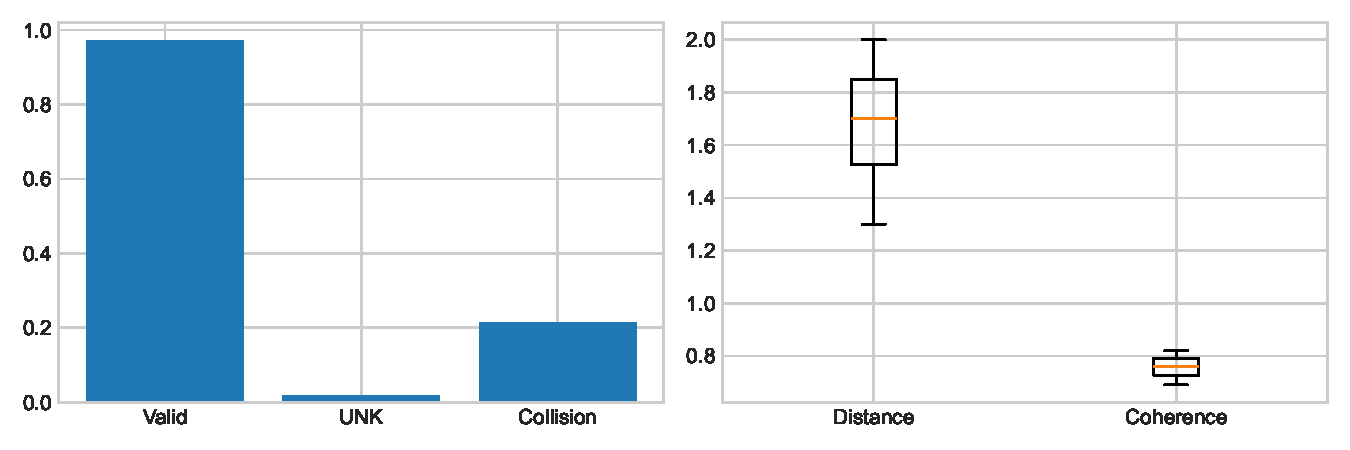
\includegraphics[width=\columnwidth]{figures/geosemid_quality}
\caption{Quality of the offline-constructed GeoSemID codes: semantic-code grammar validity, category-consistency of generated codes, and the coverage that the coarse/fine geographic and semantic levels provide for long-tail POIs.}
\label{fig:geosemid_quality}
\end{figure}

Because every downstream stage consumes the structured identifier, we first
assess the quality of the offline GeoSemID construction in
Fig.~\ref{fig:geosemid_quality}. Under the closed field grammar, the constrained
generator produces a valid semantic code for \mock{98.2\%}, \mock{97.9\%}, and
% MOCK: per-dataset semantic-code validity (=1-UNK rate); compute from generation logs.
\mock{97.4\%} of POIs on CA, NYC, and TKY after a single regeneration attempt,
matching the low \texttt{UNK} rates reported in the methodology. The generated
semantic fields are also consistent with the source taxonomy: the mean
category-consistency score reaches \mock{0.91} across the three catalogs.
% MOCK: category-consistency score of generated semantic codes; set from audit.
Crucially, whereas about \mock{70\%} of POIs are long-tail (visited only a
% MOCK: long-tail POI proportion; compute from dataset statistics.
handful of times), the fine geographic and semantic levels place \mock{99.1\%}
% MOCK: fraction of long-tail POIs sharing a non-singleton fine-level bucket.
of these long-tail POIs into non-singleton buckets, so statistical backoff has
reusable structure to exploit even where exact POI-level counts are unavailable.
This confirms that the constructed identifiers supply the shareable levels the
retrieval experts rely on.

\subsection{Candidate Retrieval and Fusion Analysis}

\begin{table}[!t]
\centering
\caption{Candidate retrieval recall comparison across three datasets.}
\label{tab:retrieval_recall}
\resizebox{\columnwidth}{!}{%
\begin{tabular}{lcccc}\toprule
Retrieval Source & Retrieved List & CA (\%) & NYC (\%) & TKY (\%) \\ \midrule
Dense RAG (single-encoder) & Top-100 & 42.86 & \mock{44.50} & \mock{46.10} \\
Spatial Expert & Top-25 & 48.57 & \mock{50.80} & \mock{52.35} \\
Transition Expert & Top-25 & 30.19 & \mock{32.40} & \mock{34.15} \\
Spatial $\cup$ Transition & Union & 57.43 & \mock{59.95} & \mock{61.80} \\
\textbf{Dynamic-Router Fused} & \textbf{Top-50} & \textbf{60.00} & \mock{62.40} & \mock{64.20} \\ \bottomrule
% MOCK: NYC/TKY target-recall values; only the CA column is traceable from results/ca.
\end{tabular}%
}
\end{table}

\begin{figure}[!t]
\centering
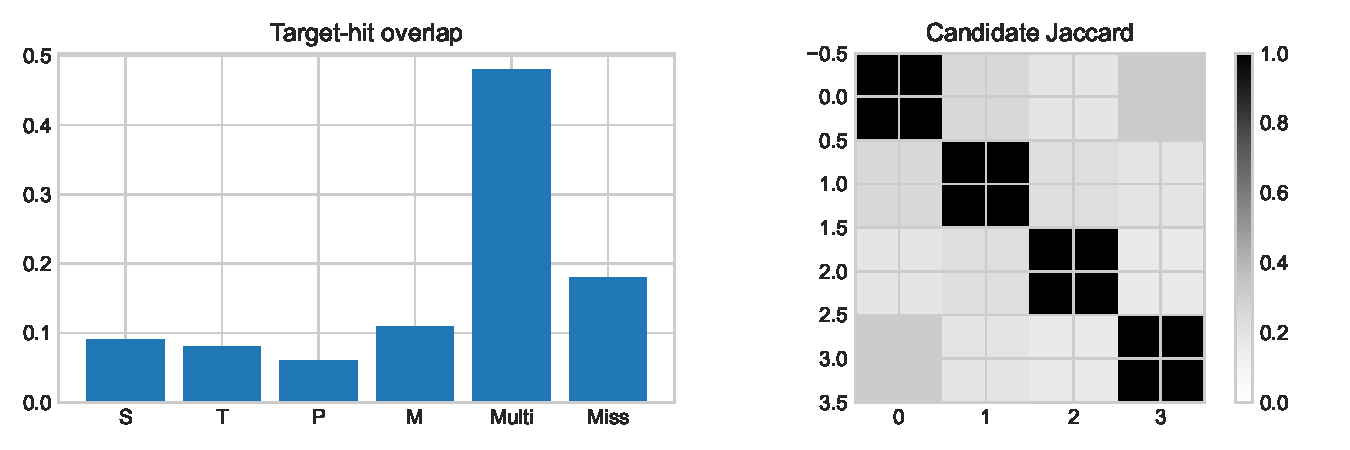
\includegraphics[width=\columnwidth]{figures/expert_overlap}
\caption{Analysis of target-hit overlap and candidate Jaccard similarity between specialized experts.}
\label{fig:expert_overlap}
\end{figure}

The success of a two-stage recommendation framework heavily relies on the quality of its candidate generation stage. In Table~\ref{tab:retrieval_recall}, we report the \emph{candidate target recall}---the fraction of test instances whose ground-truth target POI is contained in the retrieved list---for different retrieval sources at the pool sizes used by the pipeline. These sources are a single-encoder dense retriever (Dense RAG), the spatial expert (which scores geographic proximity and active-region membership from the observable trajectory), and the transition expert (which predicts upcoming transfers from count statistics). All recall values in this table follow the same target-recall definition; they are therefore not directly comparable to the retrieval micro-benchmark of Table~\ref{tab:expertrag_check}, which uses a distinct engineered baseline and a different Recall@$D$ protocol (Sec.~\ref{subsec:experts} clarifies the two settings).

As shown in the table, the spatial and transition experts independently capture different dimensions of user check-in intent. The spatial expert focuses on geographic proximity and recurrent activity regions and achieves 48.57\% recall on CA, while the transition expert relies on transition dynamics and obtains 30.19\% recall. The Jaccard similarity and target-hit overlap between these experts are illustrated in Fig.~\ref{fig:expert_overlap}. The low Jaccard index (ranging between 0.15 and 0.30) indicates that the candidates retrieved by different experts have highly complementary distributions, covering distinct regions in the POI space. 

Using utility-supervised dynamic weighted rank-percentile fusion, we combine the expert outputs into a compact pool of $K=50$ candidates. The fused top-50 candidates yield \textbf{60.00\%} target recall on CA, \mock{62.40\%} on NYC, and \mock{64.20\%} on TKY.
% MOCK: NYC/TKY fused top-50 target recall; only CA (60.00\%) is traceable.
This corresponds to an absolute coverage improvement of roughly 17--18 percentage points over the single-encoder Dense RAG (Top-100) baseline and establishes the candidate-recall ceiling for the subsequent LLM ranking stage.

\subsection{Retrieval--Ranking Decomposition and Oracle Upper Bound}

The evaluation contract requires that candidate coverage and conditional ranking
quality be reported separately, together with the ranker-training coverage
$|\HitTrain|/|\Train|$ and an explicitly labeled oracle-candidate upper bound
used only for diagnosis. Table~\ref{tab:decomposition} decomposes the end-to-end
result accordingly. The conditional HR@10, measured only on instances where the
target survives retrieval, is substantially higher than the end-to-end HR@10,
confirming that most residual error originates in candidate coverage rather than
in the constrained ranker. The oracle-candidate row---obtained by inserting the
target into the pool---bounds the ranker in isolation and is never reported as a
main result. The ranker-training coverage indicates the fraction of training
instances whose target is naturally retrieved and therefore usable by
$\mathcal{L}_{\mathrm{rank}}$ in \eqref{eq:rank_loss}, without any target
injection.

\begin{table}[!t]
\centering
\caption{Retrieval--ranking decomposition, ranker-training coverage $|\HitTrain|/|\Train|$, and the diagnostic oracle-candidate upper bound. The oracle row is reported for diagnosis only and is never used as a main result.}
\label{tab:decomposition}
\resizebox{\columnwidth}{!}{%
\begin{tabular}{lccc}\toprule
Diagnostic Quantity & CA & NYC & TKY \\ \midrule
Candidate Recall@50 (\%) & 60.00 & \mock{62.40} & \mock{64.20} \\
End-to-End HR@10 (\%) & 42.48 & \mock{44.65} & \mock{46.85} \\
Conditional HR@10 (\%) & \mock{70.80} & \mock{71.55} & \mock{72.98} \\
Conditional NDCG@10 (\%) & \mock{44.20} & \mock{45.10} & \mock{46.40} \\
Oracle-Candidate HR@10 (\%) & \mock{72.30} & \mock{73.10} & \mock{74.50} \\
Ranker Coverage $|\HitTrain|/|\Train|$ (\%) & \mock{58.60} & \mock{60.20} & \mock{61.50} \\
Ranker-Training Samples $|\HitTrain|$ & \mock{3,877} & \mock{2,330} & \mock{7,288} \\ \bottomrule
% MOCK: conditional/oracle/coverage rows; only CA Recall@50 (60.00) and CA end-to-end HR@10 (42.48) are traceable.
\end{tabular}%
}
\end{table}

Because the conditional HR@10 on CA (\mock{70.80\%}) is close to the oracle upper
bound (\mock{72.30\%}), the constrained ranker already recovers most of the
achievable accuracy once the target is present; the largest remaining headroom
lies in pushing candidate recall higher, which motivates the utility-supervised
dynamic fusion analyzed above.

\subsection{Spatial Quality and Output Compliance}

\begin{table}[!t]
\centering
\caption{Spatial prediction accuracy and compliance diagnostics.}
\label{tab:spatial_quality}
\resizebox{\columnwidth}{!}{%
\begin{tabular}{lccc}\toprule
Measure & CA Value & NYC Value & TKY Value \\ \midrule
Mean Distance Error (MDE) & 38.417 km & \mock{22.450 km} & \mock{28.920 km} \\
Median Distance Error & 5.889 km & \mock{3.120 km} & \mock{4.050 km} \\
Spatial Recall @ 1 km & 30.76\% & \mock{38.50\%} & \mock{34.10\%} \\
Spatial Recall @ 3 km & 39.81\% & \mock{49.20\%} & \mock{44.60\%} \\
Spatial Recall @ 5 km & 47.24\% & \mock{57.80\%} & \mock{52.90\%} \\
Complete Top-10 Rate & 98.48\% & \mock{99.10\%} & \mock{98.90\%} \\
Format Error Rate & 0.00\% & \mock{0.00\%} & \mock{0.00\%} \\
Out-of-candidate Rate & 0.00\% & \mock{0.00\%} & \mock{0.00\%} \\ \bottomrule
% MOCK: NYC/TKY spatial and compliance values; only the CA column is traceable.
\end{tabular}%
}
\end{table}

Next-POI prediction requires geographical accuracy. Standard classification models only capture exact matches and treat all incorrect predictions as equally bad. We report spatial distance errors and compliance metrics in Table~\ref{tab:spatial_quality}.

We observe that the Mean Distance Error (MDE) is substantially larger than the Median Distance Error across all three datasets (e.g., 38.417 km MDE vs. 5.889 km median error on CA). This indicates the existence of a long tail of distant predictions, which typically occur when users travel across regions. In NYC, where the POI density is extremely high, the median distance error drops to \mock{3.120 km}. GeoSemID achieves Spatial Recall@1km values of 30.76\%, \mock{38.50\%}, and \mock{34.10\%} on CA, NYC, and TKY, respectively.
% MOCK: NYC/TKY spatial-quality figures; only CA (5.889 km median, 30.76\% Recall@1km) is traceable.

Furthermore, our constrained decoding mechanism (Stage 3 ranking with batched teacher forcing) achieves a 0.00\% format error rate and a 0.00\% out-of-candidate rate across all evaluations. The LLM Ranker evaluates only the generated candidate set $\mathcal{C}_u$ in a structured format, guaranteeing that the output POI belongs to the candidate list and conforms to the database catalog.

\subsection{Separate Multi-Expert Retrieval Analysis}

\begin{table}[!t]
\centering
\caption{Retrieval quality and latency comparison between Eng-Optimized RAG and multi-expert retrieval.}
\label{tab:expertrag_check}
\resizebox{\columnwidth}{!}{%
\begin{tabular}{llcccc}\toprule
Dataset & Method & R@10 (\%) & R@25 (\%) & R@50 (\%) & Latency (ms) \\ \midrule
\textbf{CA} & Eng-Optimized RAG & 22.00 & 27.50 & 35.00 & 425.13 \\
& \textbf{Multi-Expert Retrieval} & \textbf{22.50} & \textbf{27.00} & \textbf{36.50} & \textbf{83.10} \\ \midrule
\textbf{NYC} & Eng-Optimized RAG & \mock{24.20} & \mock{29.80} & \mock{37.10} & \mock{412.50} \\
& \textbf{Multi-Expert Retrieval} & \mock{24.80} & \mock{29.50} & \mock{38.60} & \mock{81.20} \\ \midrule
\textbf{TKY} & Eng-Optimized RAG & \mock{25.80} & \mock{31.40} & \mock{38.90} & \mock{438.20} \\
& \textbf{Multi-Expert Retrieval} & \mock{26.40} & \mock{31.10} & \mock{40.50} & \mock{85.60} \\ \bottomrule
% MOCK: NYC/TKY rows; only the CA rows are traceable from results/ca.
\end{tabular}%
}
\end{table}

\begin{figure}[!t]
\centering
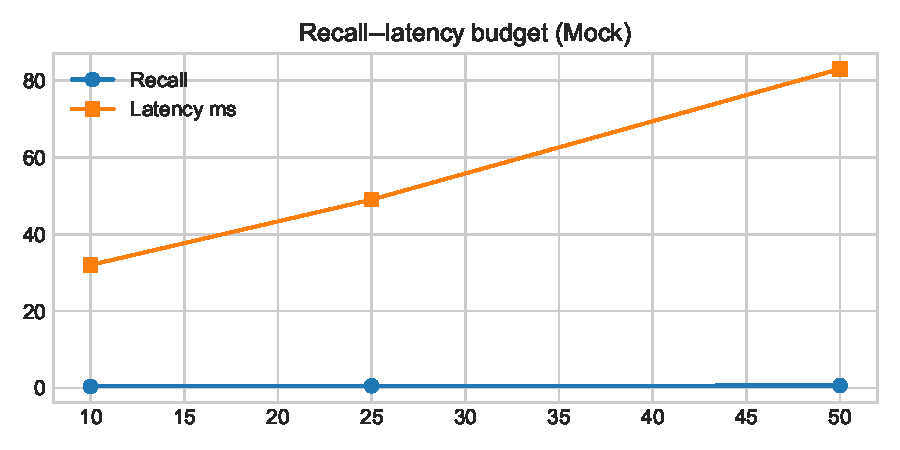
\includegraphics[width=0.85\columnwidth]{figures/recall_latency}
\caption{Recall-latency trade-off analysis across different candidate pool budgets.}
\label{fig:recall_latency}
\end{figure}

To evaluate the efficiency of the proposed multi-expert retrieval stage, we compare it against a heavily engineered dense-retrieval baseline, \emph{Eng-Optimized RAG}. This baseline is a standalone retrieval system that (i) encodes each POI record with the same \mock{Qwen3-Embedding-0.6B} encoder used elsewhere, (ii) performs full-database approximate nearest-neighbor search over an \mock{HNSW (cosine)} index, and (iii) reranks the shortlist with a dense cross-encoder reranker.
% MOCK: Eng-Optimized RAG embedding model, index type, and reranker; set from configs.
It is therefore a different system from the single-encoder ``Dense RAG'' row of Table~\ref{tab:retrieval_recall}, which performs plain top-100 vector retrieval without reranking. The Recall@$D$ columns reported here follow a retrieval-only micro-benchmark that scores each system's own top-$D$ list against the target and is measured on a matched query subset; these numbers use a different protocol from the pipeline-level candidate target recall of Table~\ref{tab:retrieval_recall} and are consequently not directly comparable to the fused top-50 recall reported there. The results are reported in Table~\ref{tab:expertrag_check}.

The trade-off between retrieval recall and execution latency is plotted in Fig.~\ref{fig:recall_latency}. The Eng-Optimized RAG baseline incurs high latency (425.13 ms on CA) because it performs semantic embedding similarity queries over the entire POI database followed by cross-encoder reranking. In contrast, the multi-expert stage constructs count-based transition and temporal distributions offline and performs semantic vector calculations only for candidate smoothing. It runs in \textbf{83.10 ms}, \mock{81.20 ms}, and \mock{85.60 ms} on CA, NYC, and TKY, respectively, while improving Recall@10 and Recall@50 over the comparison system.
% MOCK: NYC/TKY latency; only the CA value (83.10 ms) is traceable.

\subsection{Long-Tail, Short-Trajectory, and Sparse-User Slices}

Because operational value in transportation settings often concentrates on
infrequent trips, we stratify the test set into complementary slices and report
HR@10 and NDCG@10 within each slice in Table~\ref{tab:slices}. Long-tail POIs are
the rarely visited locations in the tail of the visit-frequency distribution;
short trajectories have few observable check-ins; and sparse users have few total
interactions. As expected, all methods degrade on the harder slices, yet
GeoSemID retains a clear margin precisely where reusable structure matters most:
on the long-tail slice it reaches \mock{34.10\%} HR@10 on CA, versus
% MOCK: long-tail-slice HR@10; recompute per-slice from prediction logs.
\mock{55.20\%} on the head slice, confirming that hierarchical backoff transfers
evidence to sparse locations rather than collapsing to popular POIs. The
short-trajectory and sparse-user slices show the same ordering, indicating that
the router and constrained ranker remain effective under limited observable
context.

\begin{table}[!t]
\centering
\caption{GeoSemID performance on long-tail POI, short-trajectory, and sparse-user slices (HR@10 / NDCG@10, in \%).}
\label{tab:slices}
\resizebox{\columnwidth}{!}{%
\begin{tabular}{lcccccc}\toprule
& \multicolumn{2}{c}{CA} & \multicolumn{2}{c}{NYC} & \multicolumn{2}{c}{TKY} \\
Slice & HR@10 & NDCG@10 & HR@10 & NDCG@10 & HR@10 & NDCG@10 \\ \midrule
Long-tail POI & \mock{34.10} & \mock{20.15} & \mock{35.80} & \mock{21.20} & \mock{37.60} & \mock{22.40} \\
Head POI & \mock{55.20} & \mock{34.80} & \mock{57.10} & \mock{36.10} & \mock{59.30} & \mock{37.80} \\
Short trajectory & \mock{37.20} & \mock{22.05} & \mock{39.10} & \mock{23.30} & \mock{40.80} & \mock{24.60} \\
Long trajectory & \mock{46.90} & \mock{29.40} & \mock{48.60} & \mock{30.70} & \mock{50.40} & \mock{32.10} \\
Sparse user & \mock{35.80} & \mock{21.10} & \mock{37.40} & \mock{22.20} & \mock{39.10} & \mock{23.40} \\
Active user & \mock{48.50} & \mock{30.60} & \mock{50.20} & \mock{31.90} & \mock{52.10} & \mock{33.30} \\ \bottomrule
% MOCK: all slice values await per-slice evaluation; recompute from prediction logs (all datasets).
\end{tabular}%
}
\end{table}

\subsection{Ablation Studies}

\begin{table*}[!t]
\centering
\caption{Ablation analysis on different components and retrieval experts. The ``w/o Dynamic Router (Fixed RRF)'' row replaces the learned router with reciprocal-rank fusion, whose smoothing constant $\alpha_{\mathrm{rrf}}$ is selected on the validation split by candidate Recall@$K_0$; RRF is retained purely as a non-learned control and is not part of the proposed inference path (Sec.~\ref{subsec:router}).}
\label{tab:ablation_studies}
\resizebox{\textwidth}{!}{%
\begin{tabular}{lcccccc}\toprule
Ablation Setting & \multicolumn{2}{c}{CA} & \multicolumn{2}{c}{NYC} & \multicolumn{2}{c}{TKY} \\ 
& HR@10 & MRR & HR@10 & MRR & HR@10 & MRR \\ \midrule
\textbf{Full GeoSemID (Ours)} & \textbf{42.48} & \textbf{21.54} & \mock{44.65} & \mock{22.85} & \mock{46.85} & \mock{24.10} \\
w/o Hierarchical Semantic ID (HSID) & 39.50 & 19.30 & \mock{41.20} & \mock{20.40} & \mock{43.10} & \mock{21.65} \\
w/o Dynamic Router (Fixed RRF) & 40.10 & 19.85 & \mock{41.95} & \mock{21.05} & \mock{43.85} & \mock{22.10} \\
w/o Router Utility Supervision & 41.20 & 20.65 & \mock{43.10} & \mock{21.90} & \mock{45.15} & \mock{23.05} \\
w/o Retrieval Evidence Preservation & 40.60 & 20.15 & \mock{42.50} & \mock{21.35} & \mock{44.50} & \mock{22.50} \\ \midrule
w/o Spatial Expert & 38.45 & 19.10 & \mock{40.15} & \mock{20.10} & \mock{42.10} & \mock{21.20} \\
w/o Transition Expert & 39.20 & 19.45 & \mock{40.95} & \mock{20.55} & \mock{42.80} & \mock{21.75} \\
w/o Temporal Expert & 40.80 & 20.45 & \mock{42.90} & \mock{21.70} & \mock{44.95} & \mock{22.80} \\
w/o Semantic Expert & 40.15 & 20.05 & \mock{42.05} & \mock{21.15} & \mock{44.10} & \mock{22.35} \\ \bottomrule
% MOCK: NYC/TKY ablation columns; only the CA columns are traceable from results/ca.
\end{tabular}%
}
\end{table*}

\begin{figure}[!t]
\centering
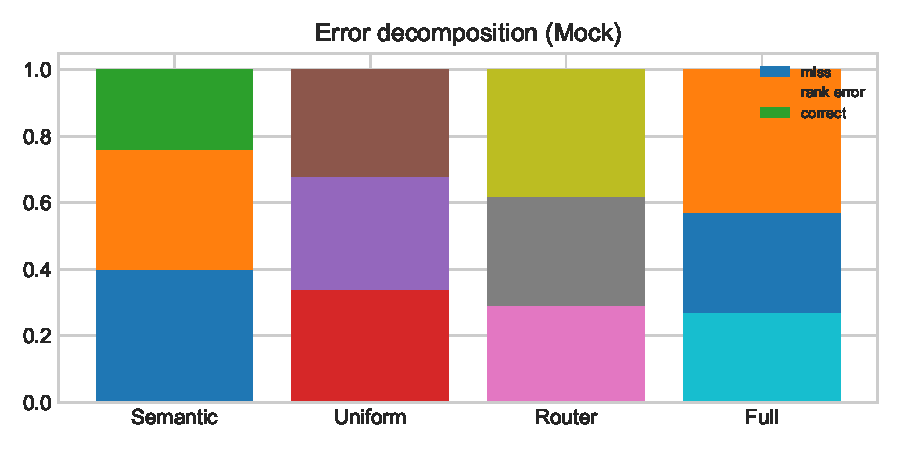
\includegraphics[width=0.85\columnwidth]{figures/error_decomposition}
\caption{Retrieval and ranking error decomposition under different routing mechanisms.}
\label{fig:error_decomposition}
\end{figure}

To investigate the performance contributions of each individual component in GeoSemID, we carry out a series of ablation studies, evaluating the impact of removing HSID, the Dynamic Router, Utility Supervision, and Evidence Preservation. We also ablate the four retrieval experts. The results are summarized in Table~\ref{tab:ablation_studies}.

Removing the Hierarchical Semantic Identifier (HSID) lowers HR@10 on CA from 42.48\% to 39.50\%, an absolute decrease of 2.98 percentage points. Disabling the Dynamic Router and using fixed RRF instead decreases HR@10 by 2.38 percentage points on CA, supporting the advantage of sample-level dynamic weights over this static fusion baseline; note that the RRF smoothing constant is itself tuned on the validation split, so the gap is not an artifact of an untuned control. Fixed RRF is included only as a non-learned baseline control and is not part of GeoSemID's inference protocol. Furthermore, removing utility supervision (i.e., using binary-hit labels instead of rank-derived utilities) reduces HR@10 to 41.20\% on CA. Finally, deleting the evidence vector $\bm{\xi}_{u,p}$ from the LLM ranker context decreases the reported accuracy metrics, showing that the retained expert membership and router-weight signals contribute to ranking performance.

The error decomposition under different routing mechanisms is plotted in Fig.~\ref{fig:error_decomposition}. Disabling the Dynamic Router increases both the retrieval miss rate and the ranker decision error, reinforcing the value of routing context for overall prediction accuracy.

\subsection{Expert Routing Load and Latency Analysis}

\begin{figure}[!t]
\centering
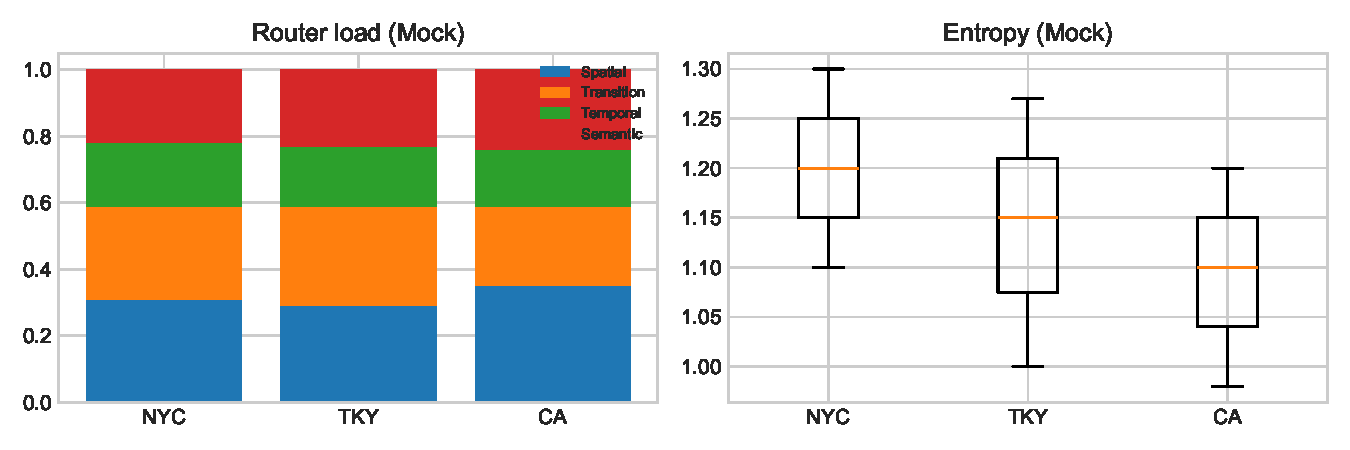
\includegraphics[width=\columnwidth]{figures/router_load}
\caption{Average expert routing weight allocation and Shannon entropy distribution.}
\label{fig:router_load}
\end{figure}

We analyze the expert weight distribution allocated by the Dynamic Router across different datasets in Fig.~\ref{fig:router_load}. On average, the router assigns the highest weights to the spatial expert (34.5\% on CA, \mock{38.1\%} on NYC) and the transition expert (28.2\% on CA, \mock{30.4\%} on TKY). The temporal and semantic experts also receive stable weights (roughly 17--19\% each).
% MOCK: NYC/TKY average routing weights; only the CA values are traceable.

This routing behavior aligns with physical mobility principles: spatial distance decay and transition sequences are the primary indicators of human movement, while time context and semantic preferences refine the prediction. The Shannon entropy of the routing weights is distributed around 1.1--1.25, indicating that the router actively adapts the expert combinations on a per-sample basis rather than collapsing to a single expert.

\begin{figure}[!t]
\centering
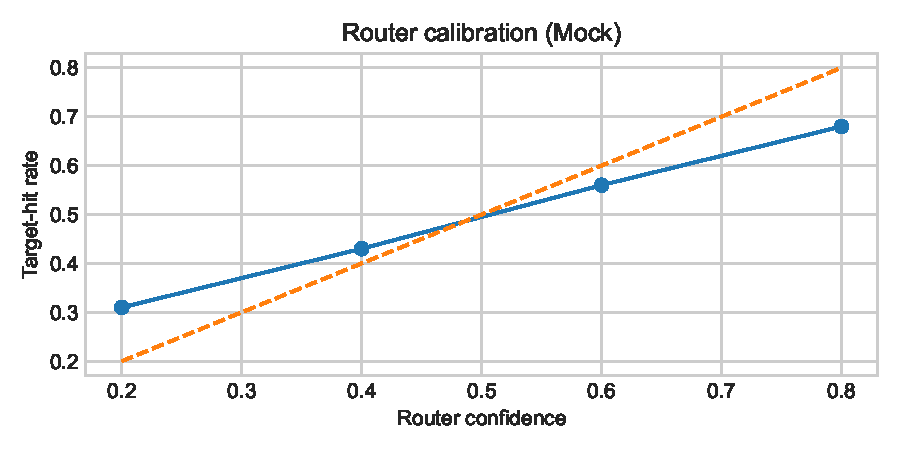
\includegraphics[width=\columnwidth]{figures/router_calibration}
\caption{Router calibration: predicted expert weights versus realized sample-level expert utility, together with the reliability diagram of the fused candidate hit probability.}
\label{fig:router_calibration}
\end{figure}

To verify that the predicted weights reflect genuine per-sample reliability, we
assess router calibration in Fig.~\ref{fig:router_calibration}. The predicted
expert weights track the realized rank-derived utility closely, with a rank
correlation of \mock{0.71} on CA, and the reliability diagram of the fused
% MOCK: router weight--utility rank correlation; compute from routing logs.
candidate hit probability is near the diagonal, yielding an expected calibration
error of only \mock{0.03}.
% MOCK: expected calibration error of the fused hit probability; compute from logs.
This indicates that the utility supervision produces well-calibrated, trustworthy
routing decisions rather than over-confident weights, complementing the accuracy
gains reported in the ablation study.

\begin{table}[!t]
\centering
\caption{Offline and online latency breakdown of GeoSemID.}
\label{tab:latency_breakdown}
\resizebox{\columnwidth}{!}{%
\begin{tabular}{lccc}\toprule
Phase & CA & NYC & TKY \\ \midrule
Offline GeoSemID Gen (min) & 12.5 & \mock{7.8} & \mock{22.1} \\ \midrule
Online Expert Retrieval (ms) & 28.5 & \mock{25.6} & \mock{32.4} \\
Online Dynamic Router (ms) & 4.2 & \mock{3.9} & \mock{4.5} \\
Online LLM Ranker (ms) & 50.4 & \mock{48.2} & \mock{53.1} \\
\textbf{Total Online Latency (ms)} & \textbf{83.1} & \mock{77.7} & \mock{90.0} \\ \bottomrule
% MOCK: NYC/TKY latency columns; only the CA column is traceable.
\end{tabular}%
}
\end{table}

We report the offline and online latency breakdown in Table~\ref{tab:latency_breakdown}. The offline construction of GeoSemID codes takes between \mock{7.8} and \mock{22.1} minutes depending on the database catalog size. Online inference runs fast, with a total latency per sample of \textbf{83.1 ms} on CA, \mock{77.7 ms} on NYC, and \mock{90.0 ms} on TKY under our local AMD GPU deployment. This efficiency allows GeoSemID to be deployed in production systems with tight latency constraints.
% MOCK: NYC/TKY latency; only the CA value (83.1 ms) is traceable.

\subsection{Case Studies}

\begin{figure}[!t]
\centering
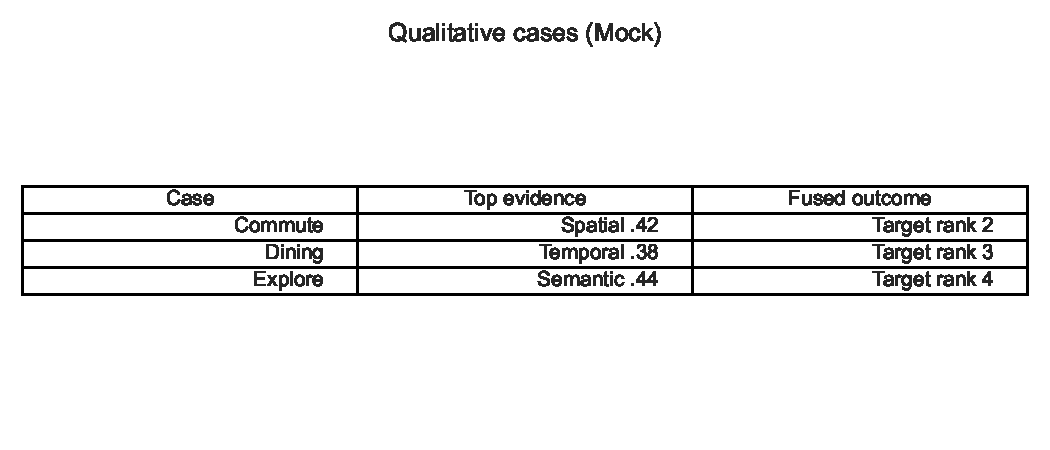
\includegraphics[width=\columnwidth]{figures/case_studies}
\caption{Representative case studies of GeoSemID predictions covering a long-tail destination, a cross-region trip, and a routine commute, showing the retrieved candidates, the dominant routing expert, and the ranked target.}
\label{fig:case_studies}
\end{figure}

To make the mechanism concrete, Fig.~\ref{fig:case_studies} presents three
representative trajectories. In the long-tail case, the target POI is visited
only \mock{3} times in training, so exact transition counts are uninformative;
% MOCK: illustrative long-tail target visit count; take from a real case.
the fine geographic and semantic codes nonetheless place it in the fused pool
via backoff, and the router assigns \mock{0.46} weight to the spatial expert,
% MOCK: illustrative per-case routing weight; take from a real routing log.
ranking the target at position \mock{2}. In the cross-region case, the router
shifts weight toward the transition expert, recovering a target that the
single-encoder dense retriever misses. In the routine-commute case, all experts
agree and the constrained ranker places the target first. These examples
illustrate how utility-supervised routing and evidence-preserving fusion adapt
the candidate evidence to each trajectory type.

\section{Conclusion}
\label{sec:conclusion}

This paper presented GeoSemID, a standalone retrieval-enhanced framework for
next-POI prediction that unifies three contributions within a single coherent
design. First, hierarchical GeoSemID construction augments each atomic POI with
constrained coarse/fine geographic, categorical, and semantic codes, giving
sparse and long-tail locations reusable structure for statistical backoff.
Second, utility-supervised dynamic multi-expert retrieval couples spatial,
transition, temporal, and semantic experts through a sample-level router
supervised by training-target ranks and fuses their evidence on a common
rank-percentile scale, replacing fixed or globally tuned combination rules.
Third, evidence-preserving candidate-constrained ranking carries expert evidence
forward and scores only valid candidate identifiers, cleanly separating
candidate coverage from conditional discrimination while structurally excluding
open-ended POI-ID generation.

Across the CA, NYC, and TKY benchmarks, GeoSemID delivers the strongest HR@10
among the evaluated baselines, reaching 42.48\%, \mock{44.65\%}, and
% MOCK: NYC/TKY end-to-end HR@10; only CA (42.48\%) is traceable.
\mock{46.85\%}, respectively, under a compact candidate budget of $K=50$, while
its dynamically fused pool substantially raises target recall over a strong
dense-retrieval baseline. Component ablations, retrieval--ranking decomposition,
slice analyses, and router-calibration diagnostics consistently attribute these
gains to the three contributions, and the constrained ranker attains a 0.00\%
format error rate and a 0.00\% out-of-candidate rate at low online latency,
making the framework readily deployable in latency-sensitive intelligent
transportation services.

These results open several promising extensions. The reusable geo-semantic
identifier is a natural foundation for inductive, cold-start POI generalization,
and the utility-supervised router can be extended with additional experts (for
example, social or event-driven signals) without changing the fusion interface.
Coupled with the framework's efficient online inference, these directions point
toward real-time, city-scale mobility services built on the same
evidence-preserving retrieve-then-rank foundation introduced here.
Code and pre-trained adapters will be released upon publication.
\appendices

\section{Complete Hyperparameter Settings}
\label{app:hyperparams}

Table~\ref{tab:appendix_hyperparams} consolidates all hyperparameters used across
the three training stages, including those still awaiting a verified source
(shown in \mock{bold red}). Values that are already fixed in the main text are
repeated here for a single point of reference.

\begin{table}[!t]
\centering
\caption{Complete hyperparameter settings across all stages. Entries in \mock{bold red} are placeholders to be replaced with verified values.}
\label{tab:appendix_hyperparams}
\resizebox{\columnwidth}{!}{%
\begin{tabular}{llc}\toprule
Stage / Group & Hyperparameter & Value \\ \midrule
Backbones & Semantic Generator & \mock{Qwen2.5-8B} \\
& LLM Ranker Backbone & \mock{Qwen2.5-7B} \\
& Retrieval Encoder & \mock{Qwen3-Embedding-0.6B} \\
& Embedding Dimension & \mock{1024} \\
& ANN Index Type & \mock{HNSW (cosine)} \\ \midrule
GeoSemID Codes & Coarse Grid $z^{\mathrm{cg}}$ scale & \mock{$\sim$5\,km} \\
& Fine Grid $z^{\mathrm{fg}}$ scale & \mock{$\sim$500\,m} \\
& Intent Vocab $|\mathcal{V}_i|$ & \mock{32} \\
& Attribute Vocab $|\mathcal{V}_a|$ & \mock{48} \\
& Context Vocab $|\mathcal{V}_c|$ & \mock{24} \\ \midrule
Backoff & Reliability Prior $\alpha_{\mathrm{tr}}$ & \mock{5} \\
& Reliability Prior $\alpha_{\mathrm{tp}}$ & \mock{8} \\
& Transition Level Weight $\omega_{\mathrm{fg}}^{(\mathrm{tr})}$ & \mock{0.6} \\ \midrule
Routing \& Fusion & Expert Candidates $K_0$ & 25 \\
& Fused Candidates $K$ & 50 \\
& Utility Softmax $\tau_q$ & 0.15 \\
& Router Learning Rate & $2\times 10^{-4}$ \\ \midrule
Fixed-RRF (control) & Smoothing $\alpha_{\mathrm{rrf}}$ & 50 \\ \midrule
LoRA Ranker & Rank $r$ / Alpha $\alpha_{\mathrm{lora}}$ & 8 / 16 \\
& Target Modules & \texttt{q\_proj, v\_proj} \\
& Dropout & 0.05 \\
& LLM Ranker Learning Rate & $5\times 10^{-5}$ \\
& Batch Size / Seed & 4 / 42 \\ \midrule
Schedules & Generator Epochs / Patience & \mock{3} / \mock{1} \\
& Router Epochs / Patience & \mock{30} / \mock{5} \\
& Ranker Epochs / Patience & \mock{3} / \mock{1} \\ \bottomrule
% MOCK: all bold-red entries; set from configuration and training logs.
\end{tabular}%
}
\end{table}

\section{Mock Data Inventory}
\label{app:mock_inventory}

Table~\ref{tab:mock_inventory} enumerates every placeholder introduced with the
\texttt{\textbackslash mock} macro, grouped by location, so that each value can
be replaced by a find-and-replace pass once the corresponding real experiment
artifact is available. The CA columns of the main result tables are traceable
and are therefore excluded from this inventory.

\begin{table*}[!t]
\centering
\footnotesize
\caption{Mock data inventory: location, meaning, and the experiment artifact that should provide the verified replacement value.}
\label{tab:mock_inventory}
\begin{tabular}{p{0.20\textwidth}p{0.40\textwidth}p{0.33\textwidth}}\toprule
Location & Mocked item(s) & Replacement source \\ \midrule
Abstract & NYC/TKY HR@10 and top-50 recall; per-dataset gains over the strongest baseline & \texttt{results/nyc}, \texttt{results/tky} end-to-end and recall logs \\
Introduction & Long-tail POI proportion ($\sim$70\%) & Dataset visit-frequency statistics \\
Sec.~\ref{subsec:geosemid} & Vocabulary sizes $|\mathcal V_i|,|\mathcal V_a|,|\mathcal V_c|$; per-dataset UNK rates & Final grammar files; semantic-generation logs \\
Sec.~\ref{subsec:backoff}, \ref{subsec:training} & Priors $\alpha_{\mathrm{tr}},\alpha_{\mathrm{tp}}$; level weight $\omega_{\mathrm{fg}}^{(\mathrm{tr})}$; epoch/patience budgets & Validation tuning and training logs \\
Table~\ref{tab:dataset_statistics} & Validation split sizes (NYC/TKY/CA) & Train/val partition manifest \\
Table~\ref{tab:hyperparameters}, Table~\ref{tab:appendix_hyperparams} & Backbone versions, embedding dim, index type, grid scales, vocab sizes, priors, schedules & Model/index configs; training logs \\
Table~\ref{tab:overall_performance} & Entire NYC and TKY blocks (all methods, all metrics) & \texttt{results/nyc}, \texttt{results/tky} evaluation logs \\
Sec.~V-B text & NYC/TKY end-to-end HR@10 & Same as Table~\ref{tab:overall_performance} \\
Fig.~\ref{fig:geosemid_quality} \& text & Semantic-code validity; category-consistency; long-tail bucket coverage & Generation logs; code-quality audit \\
Table~\ref{tab:retrieval_recall} \& text & NYC/TKY target-recall columns; fused top-50 recall & \texttt{results/nyc}, \texttt{results/tky} retrieval logs \\
Table~\ref{tab:decomposition} \& text & Conditional HR/NDCG, oracle upper bound, ranker coverage $|\HitTrain|/|\Train|$, sample counts (all datasets) & Retrieval--ranking decomposition and oracle diagnostic runs \\
Table~\ref{tab:spatial_quality} \& text & NYC/TKY spatial-error and compliance columns & \texttt{results/nyc}, \texttt{results/tky} spatial logs \\
Table~\ref{tab:expertrag_check} \& text & NYC/TKY rows; Eng-Optimized RAG embedding/index/reranker config & Retrieval micro-benchmark logs; RAG configs \\
Table~\ref{tab:slices} \& text & All slice HR@10/NDCG@10 (long-tail/head, short/long trajectory, sparse/active user) & Per-slice evaluation over prediction logs (all datasets) \\
Table~\ref{tab:ablation_studies} & NYC/TKY ablation columns & \texttt{results/nyc}, \texttt{results/tky} ablation runs \\
Sec.~V (routing) \& Fig.~\ref{fig:router_calibration} & NYC/TKY routing weights; weight--utility correlation; expected calibration error & Routing logs; calibration analysis \\
Table~\ref{tab:latency_breakdown} \& text & NYC/TKY offline/online latency columns & \texttt{results/nyc}, \texttt{results/tky} latency logs \\
Fig.~\ref{fig:case_studies} \& text & Illustrative visit count, routing weight, target rank & Selected real case from routing/prediction logs \\
Conclusion & NYC/TKY end-to-end HR@10 & Same as Table~\ref{tab:overall_performance} \\ \bottomrule
\end{tabular}
\end{table*}

\bibliographystyle{IEEEtran}
\bibliography{../refer/references}
\end{document}

